%!TEX root =../MemoriaTFM.tex
%El anterior comando permite compilar este documento llamando al documento raíz
\chapter{Entorno de trabajo}\label{chp-03}
\epigraph{Technology is nothing. What's important is that you have a faith in people, that they're basically good and smart, and if you give them tools, they'll do wonderful things with them.}{Steve Jobs, 1994\\Businessman}

\lettrine[lraise=-0.1, lines=2, loversize=0.2]{A}{ntes} de comenzar el proceso de desarrollo de la parte técnica de la memoria es necesario preparar un entorno adecuado de trabajo, es decir, un conjunto de herramientas hardware y software que permitan llevar a cabo el proyecto con la mayor comodidad y precisión posible.

La correcta elección de un entorno de trabajo adecuado es fundamental a la hora de abordar cualquier tipo de proyecto, ya que el éxito o fracaso, o al menos la eficiencia del proceso de desarrollo del mismo, va a depender en gran medida de dicho entorno utilizado.
El apartado actual presenta el entorno de trabajo utilizado para la realización de este \gls{TFM}.

\section{Git y GitHub}

Los sistemas de control de versiones son programas cuyo principal objetivo es controlar los cambios producidos en el desarrollo de cualquier tipo de software, permitiendo conocer el estado actual de un proyecto, las personas que intervinieron en ellos, etc. Un buen control de versiones es tarea fundamental para la administración de un proyecto de desarrollo de software en general\cite{alcazar2014}. Git es uno de los sistemas de control de versiones más populares entre los desarrolladores, es gratuito, open source, rápido y eficiente, aunque gran parte su popularidad es debido a GitHub(\autoref{jenkins-logo}), un excelente servicio de alojamiento de repositorios de software que ofrece un amplio conjunto de características de gran utiilidad para el trabajo en equipo.

\begin{figure}[htbp]
	\centering
	
\includegraphics[width=0.80\linewidth]
	{entorno/figuras/github.png}
	\caption{Logotipo de GitHub}
	\label{github-logo}
\end{figure}

A continuación se muestran algunas de las características que han llevado a GitHub a ser tan valorado entre los desarrolladores\cite{quintana2015}:

\begin{itemize}
	\item Permite versionar el código, es decir, guardar en determinado momento los cambios realizados sobre un archivo o conjunto de archivos con la oportunidad de tener acceso al historial de cambios al completo, bien para regresar a alguna de las versiones anteriores o bien para poder realizar comparaciones entre ellas.
	\item Gracias a la gran cantidad de repositorios de \gls{SW} públicos que alberga, es posible leer, estudiar y aprender de el código creado por miles de desarrolladores en el mundo, permitiendo incluso la oportunidad de adaptarlos a las necesidades propias de cada desarrollador, sin alterar el original y realizando una copia o fork\footnote{Copia exacta en crudo del repositorio original que podrá ser utilizada como un repositorio git cualquiera} de este.
	\item Tras haber realizado un fork de un proyecto y haber realizado algunos ajuste, introducido alguna mejora o arreglado algún problema que pudiera contener, es posible integrar los cambios realizados al proyecto original (previa supervisión de su propietario, administrador o alguno de sus colaboradores), por lo que un repositorio puede llegar a ser construido mediante la contribución de una gran comunidad de desarrolladores.
	\item GitHub posee un sistema propio de notificaciones con el que poder estar informado de lo que ocurre en torno a un repositorio concreto, ya sea privado a la compañía o público a la comunidad.
	\item GitHub trae incorporado un visor de código, mediante el cual (y a través del navegador) es posible consultar el contenido de un archivo determinado, con la sintaxis correspondiente al lenguaje utilizado y sin necesidad de descargar una copia del mismo.
	\item Cada repositorio de \gls{SW} albergado en GitHub cuenta con su propio seguimiento de incidencias, con un elaborado sistema de tickets, de manera tal que cualquier colaborador (o usuario en general) pueda reportar algún problema encontrado en la utilización el código o pueda simplemente sugerir nuevas características para que sean implementadas.
	\item Al ser una plataforma web es totalmente independiente al \gls{SO} utilizado, siendo por otro lado Git compatible con los principales sistemas actuales: Linux, Windows, OSX.
	\item GitHub es gratuito e ilimitado para repositorios de proyectos públicos, sólo aquellos usuarios que deseen mantener proyectos en privado deberán pagar una cuota. 
\end{itemize}

\TODO{TODO - Una frase de cierre al apartado}


\section{Bundler-audit}

Como ya fue comentado en el apartado \ref{dependencias} cada aplicación tiene sus dependencia, las que a su vez pueden contener vulnerabilidades de seguridad. Encontrar las vulnerabilidades de seguridad que presenta una aplicación es una tarea necesaria y tediosa, que de ser obviada no impedirá que la aplicación generada siga siendo ejecutada como si todo estuviera funcionando en perfectas condiciones, pero que ocultará agujeros en la aplicación que podrán ser utilizados en diversa manera por algún usuario malintencionado.

Para cualquier aplicación escrita con Ruby y en ausencia de alguna herramienta automatizada de análisis de vulnerabilidades, el desarrollador del código deberá estar suscrito a cada lista de correo relacionada con anuncios de seguridad de dependencias y realizar un seguimiento exclusivo de vulnerabilidades y actualizaciones de seguridad de cada una de las dependencias incluidas en la aplicación, para cada aplicación en la que participe\cite{prescott2015}.

Por el contrario, todo este proceso puede ser automatizado en Ruby gracias a bundler-audit\cite{bundleaudit2017}, del grupo de colaboradores Rubysec, un verificador a nivel de parche para Bundler\footnote{Bundler es la herramienta Ruby para el manejo de dependencias, mantenidas en los archivos Gemfile y Gemfile.lock.} con las siguientes características:

\begin{itemize}
	\item bundler-audit analiza las vulnerabilidades en las versiones de las gemas contenidas en el archivo de dependencias \textit{Gemfile.lock} de la aplicación.
	\item Analiza las fuentes de dependencias que puedan ser inseguras (http://).
	\item Permite especificar avisos de seguridad que serán ignorados en el análisis\todo{iNCLUIR ESTO EN LAS PRUEBAS}, bien por ser un riesgo asumido por el desarrollador, una vulnerabilidad ya conocida y en la que se está actualmente trabajando o cualquier otro motivo.
	\item No requiere de conexión a internet para cada ejecución que se realice del análisis.
	\item Funciona cruzando la información de dependencias recogidas del fichero \textit{Gemfile.lock} con una lista de vulnerabilidades conocidas\cite{advisorydb2017}, basada en información pública existente en bases de datos como \gls{CVE}\footnote{Lista de información registrada sobre vulnerabilidades conocidas, definida y mantenida por The MITRE Corporation}.
\end{itemize}

El código \ref{prg03-01} muestra un ejemplo del resultado obtenido a la salida del terminal de comandos al realizar un análisis estático de vulnerabilidades con bundler-audit al archivo \textit{Gemfile.lock} de un proyecto:

\begin{lstlisting}[language=,caption={Ejemplo de uso de bundler-audit}, breaklines=true, label=prg03-01]
$ bundle audit
Name: actionpack
Version: 3.2.10
Advisory: OSVDB-91452
Criticality: Medium
URL: http://www.osvdb.org/show/osvdb/91452
Title: XSS vulnerability in sanitize_css in Action Pack
Solution: upgrade to ~> 2.3.18, ~> 3.1.12, >= 3.2.13

Name: actionpack
Version: 3.2.10
Advisory: OSVDB-89026
Criticality: High
URL: http://osvdb.org/show/osvdb/89026
Title: Ruby on Rails params_parser.rb Action Pack Type Casting Parameter Parsing Remote Code Execution
Solution: upgrade to ~> 2.3.15, ~> 3.0.19, ~> 3.1.10, >= 3.2.11

Name: activerecord
Version: 3.2.10
Advisory: OSVDB-90072
Criticality: Medium
URL: http://direct.osvdb.org/show/osvdb/90072
Title: Ruby on Rails Active Record attr_protected Method Bypass
Solution: upgrade to ~> 2.3.17, ~> 3.1.11, >= 3.2.12

Name: activerecord
Version: 3.2.10
Advisory: OSVDB-89025
Criticality: High
URL: http://osvdb.org/show/osvdb/89025
Title: Ruby on Rails Active Record JSON Parameter Parsing Query Bypass
Solution: upgrade to ~> 2.3.16, ~> 3.0.19, ~> 3.1.10, >= 3.2.11

Unpatched versions found!
\end{lstlisting}

Además, bundler-audit permite actualizar la base de datos ruby-advisory-db y analizar el fichero \textit{Gemfile.lock} desde el mismo comando, habilidad que resulta de gran utilidad para su ejecución en sistemas de \gls{IC}, como muestra el código \ref{prg03-02}:

\begin{lstlisting}[language=,caption={Ejecutando bundler-audit tras la actualización de las vulnerabilidades conocidas}, breaklines=true, label=prg03-02]
$ bundle audit check --update
\end{lstlisting}

Por último, y como ya se ha mencionado con anterioridad en este apartado, es posible ignorar advertencias especificadas (código \ref{prg03-03}) por el usuario:

\begin{lstlisting}[language=,caption={Ignorar vulnerabilidades con bundler-audit}, breaklines=true, label=prg03-03]
$ bundle audit check --ignore OSVDB-108664
\end{lstlisting}


\TODO{TODO - Cierre del apartado. de Rubysec para proyectos Ruby}

\section{Nsp}

Nsp es la principal herramienta de interfaz de línea de comandos de Node Security Platform y es una de las herramientas más utilizadas para monitorizar la seguridad en aplicaciones node, permitiendo auditar el archivo \textit{package.json} de dependencias de la misma.

\begin{figure}[htbp]
	\centering
	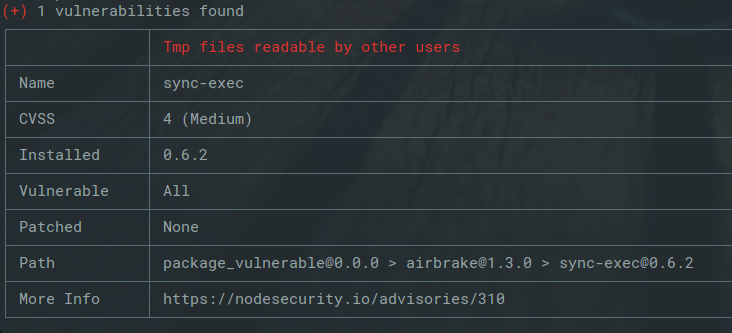
\includegraphics[width=0.80\linewidth]
	{entorno/figuras/nsp.png}
	\caption{Escaneo de vulnerabilidades en las dependencias de Node JS}
	\label{nsp-check}
\end{figure}

Su utilización es simple, permitiendo incluso ignorar vulnerabilidades que puedan estar siendo tratadas en el momento del análisis y realizando consultas contra una base de datos de vulnerabilidades mantenida por Node Security Platform, que contiene información recopilada de múltiples fuentes (por ejemplo \gls{CVE}). Basta con \textit{"nsp check"} para analizar las vulnerabilidades de la aplicación, recibiendo un resultado como el mostrado en la \autoref{nsp-check}.


\section{Docker}

\begin{figure}[htbp]
	\centering
	
\includegraphics[width=0.80\linewidth]
	{entorno/figuras/Docker.png}
	\caption{Logotipo de Docker}
	\label{docker-logo}
\end{figure}

Docker (\autoref{docker-logo}) es una herramienta de virtualización diseñada para aportar beneficios a desarrolladores, testers y administradores de sistemas, creando contenedores ligeros y portables para que las aplicaciones puedan ser ejecutadas en cualquier máquina, con sólo tener docker instalado e independientemente del \gls{SO} de la propia máquina que lo contenga\cite{garciaoterino2015}. Esta plataforma de código abierto hace uso de las funciones de aislamiento de recursos que provee el kernel de Linux para dar lugar a contenedores independientes, dentro de los cuales se ejecutará una única aplicación con sus respectivas dependencias, funcionando siempre con este único kernel, en lugar de virtualizar uno por cada contenedor o máquina virtual.

\TODO{La tecnología Docker fue creada al principio por encima de la tecnología LXC (que la mayoría de las personas relacionan con los contenedores Linux "tradicionales"), aunque se ha alejado de esa dependencia. LXC fue útil como virtualización ligera, pero no contaba con un gran desarrollador o una experiencia de usuario. La tecnología Docker proporciona más que la capacidad de ejecutar contenedores, también facilita el proceso de creación y diseño de contenedores mediante el envío de imágenes y versionado de imágenes (entre otras cosas) Añadir IMAGEN DOCKER-ESQUEMA}

Gracias al uso de docker dos desarrolladores no tendrán que, por ejemplo, preocuparse de la versión Java que cada uno tenga instalado en su propia máquina durante el desarrollo de la aplicación, ya que está podrá ser enviada de uno a otro en el interior de un contenedor, que funcionará de la misma manera en cualquiera de los dos entornos.

Además, virtualizar con docker ofrece una serie de ventajas respecto a hacerlo con máquinas virtuales convencionales\cite{velazco2016}:

\begin{itemize}
	\item \textbf{Portabilidad.} Los contenedores son portables, por lo que pueden ser trasladados fácilmente a cualquier otro equipo con Docker sin tener que volver a configurar nada.
	\item \textbf{Ligereza.} Al no virtualizar un sistema completo, sino solo lo necesario, el consumo de recursos es muy inferior.
	\item \textbf{Autosuficiencia.} Docker se encarga de todo de organizarlo todo, por lo que los contenedores tan solo deben tener lo necesario para que la aplicación funcione.
\end{itemize}

Un sistema de contenedores Docker lo componen principalmente 5 elementos fundamentales:

\begin{itemize}
	\item \textbf{Demonio:} proceso principal de la plataforma.
	\item \textbf{Cliente:} binario que constituye la interfaz al usuario y le permite interactuar con el Demonio.
	\item \textbf{Imagen:} Plantilla utilizada para crear el contenedor de la aplicación que se va a ejecutar en su interior. Dicha plantilla recibe el nombre por defecto de \textit{Dockerfile}.
	\item \textbf{Registros:} Directorios donde se almacenan las imágenes, tanto de acceso público como privado y similares a los utilizados por Linux, donde los usuarios publican sus propios contenedores de manera que aquellos otros usuarios que los necesiten puedan descargarlos directamente desde allí.
	\item \textbf{Contenedores:} Donde se almacena todo lo necesario (librerías, dependencias, binarios de la aplicación, etc.) para que la aplicación pueda ejecutarse de forma aislada.
\end{itemize}

Actualmente existen multitud de empresas que utilizan a docker como sistema de contenedores en sus centros de datos (Spotify, eBay, PayPal, etc.) y cuenta con el apoyo de grandes compañías de internet como Amazon o Google, lo que permite que Docker se encuentre en un proceso continuo de crecimiento y mejora.


\section{Clair y Clairctl}

Clair (\autoref{clair-logo}) es un proyecto de código libre desarrollado por CoreOS para el análisis estático de vulnerabilidades en contenedores de aplicaciones, que funciona de la siguiente manera\cite{clair2017}:

\begin{figure}[htbp]
	\centering
	
\includegraphics[width=0.80\linewidth]
	{entorno/figuras/clair.png}
	\caption{Clair}
	\label{clair-logo}
\end{figure}

\begin{enumerate}
	\item A intervalos regulares, Clair realiza una ingesta de metadatos de vulnerabilidad desde un conjunto configurado de fuentes \TODO{VER QUE MAS FUENTES APARTE DE CVE ESTAN UTILIZANDO} y los almacena en una base de datos PostgreSQL.
	\item Un cliente configurado para utilizar la \gls{API} de Clair indexa y escanea sus imágenes de contenedores por capas, creando una lista de características presentes en la imagen y almacenándolas en la base de datos.
	\item El cliente solicita a través de la \gls{API} a la base de datos las vulnerabilidades conocidas para una imagen en particular, correlacionando las vulnerabilidades y características de la imagen, de manera que esta no requiere un escaneo completo para cada petición.
	\item En caso de que se produzcan actualizaciones para los metadatos de vulnerabilidad, se enviará una notificación que alertará a los sistemas de que se ha producido un cambio, siendo escaneada de nuevo la imagen la próxima vez que sea solicitado un informe.
\end{enumerate}

Por otro lado, Clairctl es uno de los clientes más utilizados para alcanzar la \gls{API} de Clair y se caracteriza por ser una herramienta ligera de interfaz de comandos y escrita en el lenguaje de programación desarrollado por Google, Go. Clairctl es capaz de hacer de puente entre registros de imágenes tales como Docker Hub, Docker Registry o Quay.io (registro de imágenes de CoreOS). La \autoref{clair-esquema} muestra el esquema resultado de utilizar ambas herramientas para el análisis estático de contenedores de aplicaciones.

\begin{figure}[htbp]
	\centering
	
\includegraphics[width=0.80\linewidth]
	{figuras/emplazamiento-imagen.png}
	\caption{Esquema de escaneo y detección de vulnerabilidades en imágenes Docker}
	\label{clair-esquema}
\end{figure}

\section{Jenkins \gls{CI}}

Jenkins \gls{CI} (\autoref{jenkins-logo}) es una herramienta autónoma de código abierto que puede utilizarse para automatizar todo tipo de tareas, como la construcción, prueba y despliegue de software. Jenkins puede ser instalado a través de paquetes de sistemas nativos, Docker, o incluso ser ejecutado de manera independiente en cualquier máquina con el entorno de ejecución de Java instalado\cite{jenkins2017}.


\begin{figure}[htbp]
	\centering
	
\includegraphics[width=0.80\linewidth]
	{entorno/figuras/jenkins.png}
	\caption{\gls{IC} con Jenkins}
	\label{jenkins-logo}
\end{figure}

Jenkins posee, entre otras, las siguientes ventajas:

\begin{itemize}
	\item \textbf{Integración Continua y Despliegue Continuo}: Al ser un servidor de automatización extensible, Jenkins puede ser utilizado simplemente como un servidor de \gls{IC} o convertirse en un entorno completo de \gls{IC} y \gls{DC} para cualquier tipo de proyecto.
	\item \textbf{Fácil instalación}: Jenkins es una aplicación auto-contenida diseñada con Java, lista para ser ejecutada y empaquetada para los \gls{SO} Windows y Mac OSX, así como cualquier sistema Unix.
	\item \textbf{Fácil configuración}: Jenkins aporta una configuración mediante interfaz web de fácil manejo, que incluye análisis instantáneos de errores y ayuda en compilaciones.
	\item \textbf{Extensible}: Jenkins dispone de cientos de plugins en su centro de actualizaciones, capaz de ser integrados prácticamente con cualquier herramienta necesaria en los procesos de integración continua y despliegue continuo.
	\item \textbf{Distribuido}: Jenkins puede distribuir fácilmente el trabajo en varias máquinas, lo que ayuda a generar mejoras, pruebas y despliegues en varias plataformas rápidamente.
	\item \textbf{Open Source}: Es una herramienta de código libre con el apoyo de una gran comunidad.
	\item \textbf{Soporte de repositorio de control de versiones}: Gracias a Jenkins, el código puede ser descargado directamente desde un repositorio de contro de versiones (GitHub, BitBucket, etc.) con multitud de opciones.
	\item \textbf{Soporte de scripts}: Puede ejecutar scripts de bash, shell, ANT y proyectos Maven.
	\item \textbf{Notificaciones}: Jenkins puede ser utilizado para publicar resultados y enviar emails de notificación de los mismos.
\end{itemize}

\TODO{Pipeline - A user-defined model of a continuous delivery pipeline, for more read the Pipeline chapter in this handbook.\\Debo poner también la imagen de una pipeline de trabajo con verdes y rojos.}

\section{Slack}

Slack (\autoref{slack-logo}) es una herramienta de mensajería en tiempo real diseñada para usarla en grupo, facilitando la gestión de los propios grupos de trabajo dentro del entorno de una empresa y centralizando la comunicación interna a la misma\cite{santamaria2015}. Además, permite la creación de grupos de trabajo con un número ilimitado de miembros, a la vez que es posible establecer canales de comunicación públicos, conversaciones privadas y compartir ficheros.

\begin{figure}[htbp]
	\centering
	
\includegraphics[width=0.80\linewidth]
	{entorno/figuras/Slack.png}
	\caption{Slack}
	\label{slack-logo}
\end{figure}

Por otro lado, Slack permite a sus usuarios trabajar con otros servicios basados en la web, amplificando aún más el trabajo colaborativo y proveyendo integración con múltiples herramientas de uso habitual: Dropbox, Trello, Google Drive, GitHub y Jenkins entre otras.

\TODO{TODO - ¿Cierre al apartado?}

\endinput